\chapter{Introducci\'on}
\section{Mapa mental}

Las Matemáticas en Reversa son un campo de la Lógica Matemática que se dedica a estudiar qué axiomas son necesarios y suficientes para demostrar los teoremas de la matemática clásica. A diferencia del método deductivo tradicional, que parte de los axiomas para probar un teorema, esta área realiza el proceso inverso: comienza con un teorema conocido y busca los axiomas más débiles que lo pueden demostrar.

El objetivo principal de las matemáticas en reversa es medir la complejidad de los teoremas y guiar el desarrollo de las teorías matemáticas, estableciendo una jerarquía de la fuerza axiomática.

Para lograr este objetivo, la disciplina se basa en los fundamentos de la Teoría de la Computabilidad y la Lógica Matemática, analizando qué teoremas pueden ser demostrados con métodos constructivos y cuáles requieren principios más fuertes.

La tesis se centrará en tres de los cinco principales subsistemas de las matemáticas en reversa, que sirven como puntos de referencia para clasificar los teoremas:
\begin{enumerate}
    \item $\operatorname{RCA}_{0}$ (Axiomas de Comprensión Recursiva): Considerado el sistema base o ``semilla", es un sistema débil y constructivo que se relaciona directamente con la noción de lo computable. 
    \item $\operatorname{WKL}_{0}$ (Lema Débil de K\"{o}nig): Es un sistema más fuerte que $\operatorname{RCA}_{0}$ y se vincula con el concepto de compacidad y las propiedades de los árboles infinitos.
    \item $\operatorname{ACA}_{0}$ (Axiomas de Comprensión Aritmética): Un sistema significativamente más fuerte que los anteriores, relacionado con la definibilidad y la complejidad de los conjuntos ya no necesariamente computables.

\end{enumerate}
Finalmente, se aplicará este marco teórico para analizar teoremas del Análisis Real, tales como el teorema del Valor Intermedio, el teorema de Heine-Borel, y el de Bolzano-Weierstra\ss, con el fin de determinar con precisión la fuerza axiomática que cada uno requiere para ser demostrado. (figura \ref{fig:mapa_mental})
\begin{figure}[h]
    \centering
    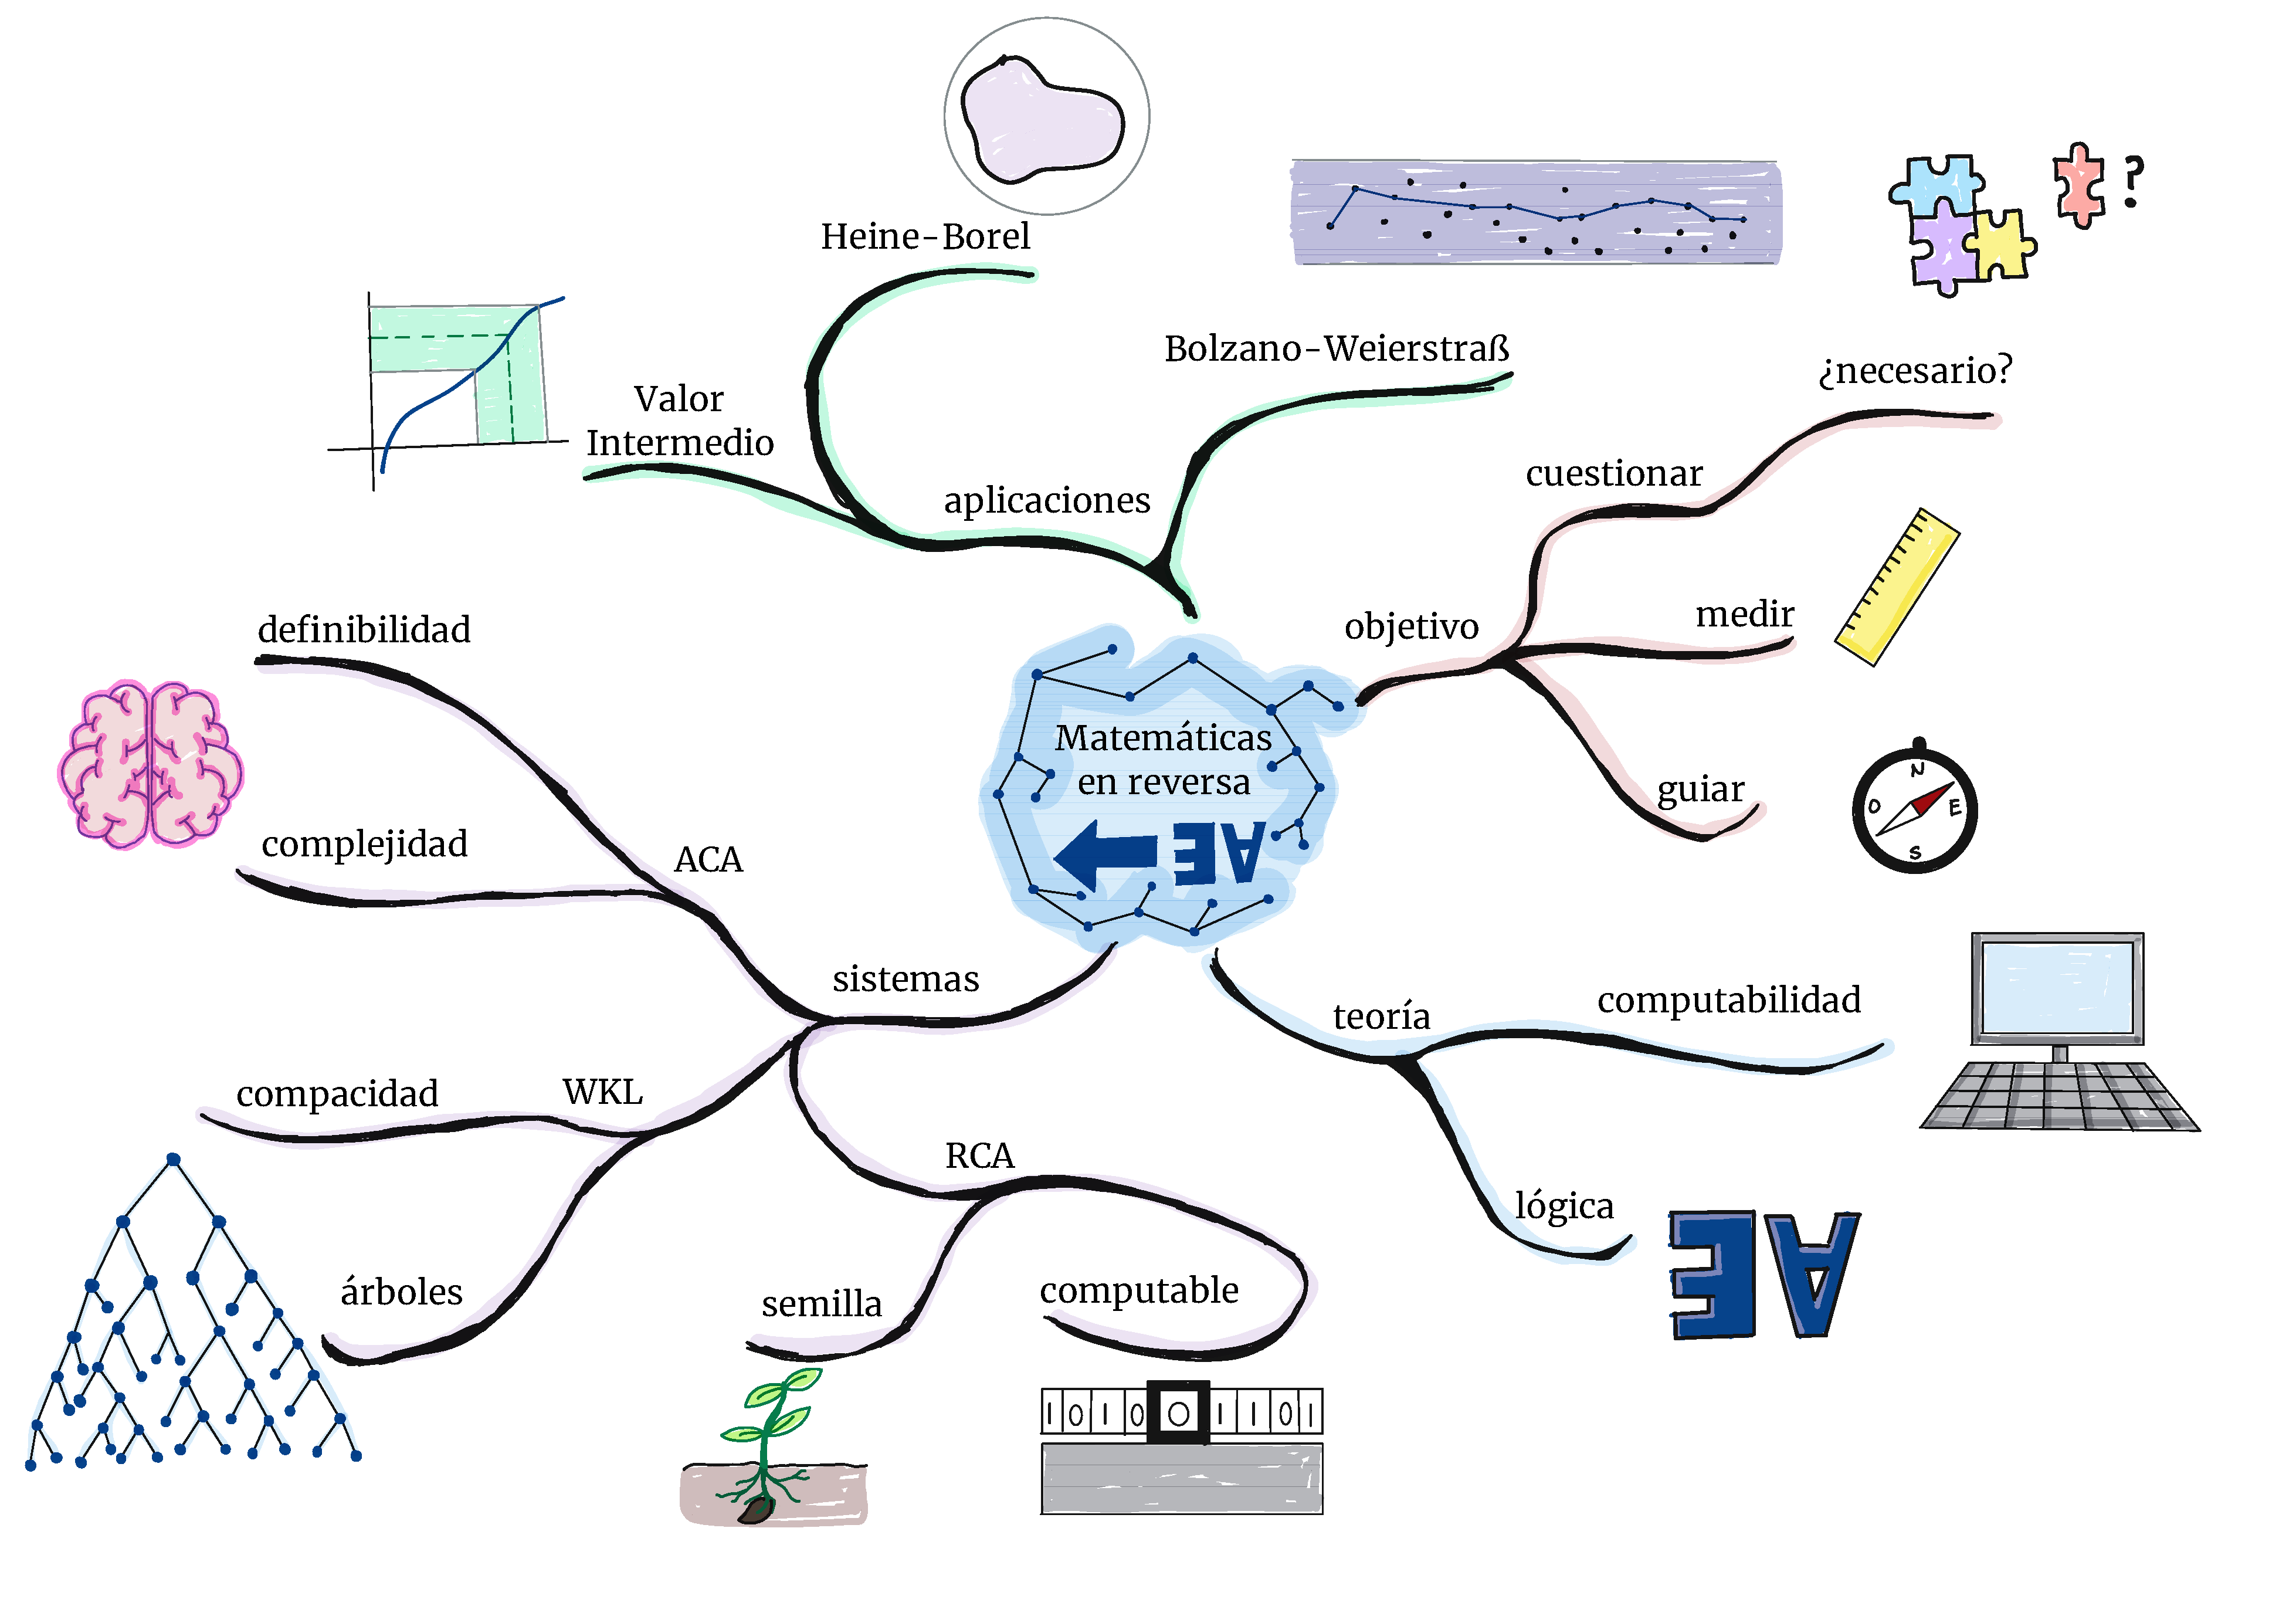
\includegraphics[width=\linewidth]{imagenes/Mapa mental.pdf}
    \caption{Mapa mental}
    \label{fig:mapa_mental}
\end{figure}

\section{Pirámide conceptual}
Se presenta a continuación una propuesta para la pirámide conceptual. Esta propuesta se enfoca en los conceptos y subconceptos de las áreas más importantes de las matemáticas en reversa, las cuales son las áreas de Lógica matemática y la Teoría de la Computabilidad.



\begin{figure}[h]
    \centering
    


\tikzset{every picture/.style={line width=0.75pt}} %set default line width to 0.75pt        

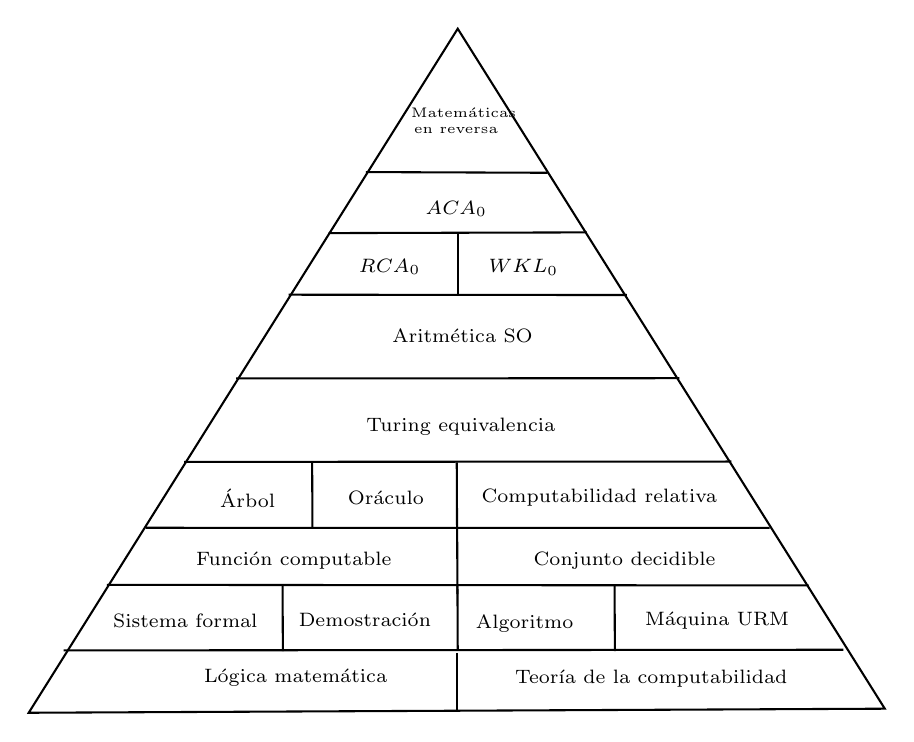
\begin{tikzpicture}[x=0.75pt,y=0.75pt,yscale=-1,xscale=1]
%uncomment if require: \path (0,370); %set diagram left start at 0, and has height of 370

%Straight Lines [id:da3672823312125487] 
\draw    (43.99,351.92) -- (456.45,349.96) -- (250.69,22.35) -- cycle ;
%Straight Lines [id:da002643119061223942] 
\draw    (60.81,321.88) -- (436.54,321.56) ;
%Straight Lines [id:da06072037866543012] 
\draw    (81.63,290.3) -- (419.75,290.57) ;
%Straight Lines [id:da7933758557929139] 
\draw    (100.43,262.8) -- (400.95,262.81) ;
%Straight Lines [id:da8802918820846337] 
\draw    (118.9,231.05) -- (382.49,230.88) ;
%Straight Lines [id:da5379646552962222] 
\draw    (143.94,190.84) -- (357.44,190.73) ;
%Straight Lines [id:da7016527384053687] 
\draw    (169.19,150.5) -- (332.2,150.66) ;
%Straight Lines [id:da5693266617663577] 
\draw    (188.43,120.82) -- (312.95,120.48) ;
%Straight Lines [id:da5134711901465621] 
\draw    (206.45,91.42) -- (293.99,91.76) ;
%Straight Lines [id:da9821515494391937] 
\draw    (250.22,323.08) -- (250.22,350.94) ;
%Straight Lines [id:da7120191972113731] 
\draw    (166.3,290.62) -- (166.44,322.19) ;
%Straight Lines [id:da02486951616469968] 
\draw    (250.55,290.36) -- (250.69,321.93) ;
%Straight Lines [id:da7634857600858367] 
\draw    (326.26,290.62) -- (326.4,322.19) ;
%Straight Lines [id:da9396590708936965] 
\draw    (250.41,263.23) -- (250.55,294.8) ;
%Straight Lines [id:da9759690725869936] 
\draw    (180.55,231.1) -- (180.69,262.67) ;
%Straight Lines [id:da42935866523306043] 
\draw    (250.22,231.28) -- (250.36,262.85) ;
%Straight Lines [id:da4820217119427046] 
\draw    (250.69,120.65) -- (250.69,150.58) ;

% Text Node
\draw (126.95,329.45) node [anchor=north west][inner sep=0.75pt]  [font=\scriptsize] [align=left] {Lógica matemática};
% Text Node
\draw (276.83,330.03) node [anchor=north west][inner sep=0.75pt]  [font=\scriptsize] [align=left] {Teoría de la computabilidad};
% Text Node
\draw (83.13,302.82) node [anchor=north west][inner sep=0.75pt]  [font=\scriptsize] [align=left] {Sistema formal};
% Text Node
\draw (172.63,302.52) node [anchor=north west][inner sep=0.75pt]  [font=\scriptsize] [align=left] {Demostración};
% Text Node
\draw (257.97,303.25) node [anchor=north west][inner sep=0.75pt]  [font=\scriptsize] [align=left] {Algoritmo};
% Text Node
\draw (339.42,301.99) node [anchor=north west][inner sep=0.75pt]  [font=\scriptsize] [align=left] {Máquina URM};
% Text Node
\draw (123.18,273.03) node [anchor=north west][inner sep=0.75pt]  [font=\scriptsize] [align=left] {Función computable};
% Text Node
\draw (285.78,273.05) node [anchor=north west][inner sep=0.75pt]  [font=\scriptsize] [align=left] {Conjunto decidible};
% Text Node
\draw (217.69,165.53) node [anchor=north west][inner sep=0.75pt]  [font=\scriptsize] [align=left] {Aritmética SO};
% Text Node
\draw (134.7,242.75) node [anchor=north west][inner sep=0.75pt]  [font=\scriptsize] [align=left] {Árbol};
% Text Node
\draw (196.24,243.58) node [anchor=north west][inner sep=0.75pt]  [font=\scriptsize] [align=left] {Oráculo};
% Text Node
\draw (260.68,242.64) node [anchor=north west][inner sep=0.75pt]  [font=\scriptsize] [align=left] {Computabilidad relativa};
% Text Node
\draw (205.19,208.67) node [anchor=north west][inner sep=0.75pt]  [font=\scriptsize] [align=left] {Turing equivalencia};
% Text Node
\draw (201.62,131.74) node [anchor=north west][inner sep=0.75pt]  [font=\scriptsize]  {$\operatorname{RCA}_{0}$};
% Text Node
\draw (264.03,132.01) node [anchor=north west][inner sep=0.75pt]  [font=\scriptsize]  {$\operatorname{WKL}_{0}$};
% Text Node
\draw (233.72,103.83) node [anchor=north west][inner sep=0.75pt]  [font=\scriptsize]  {$\operatorname{ACA}_{0}$};
% Text Node
\draw (226.72,55.39) node [anchor=north west][inner sep=0.75pt]  [font=\tiny] [align=left] {\begin{minipage}[lt]{32.52pt}\setlength\topsep{0pt}
\begin{center}
Matemáticas en reversa
\end{center}

\end{minipage}};


\end{tikzpicture}

    \caption{Pirámide conceptual}
    \label{fig: piramide_conceptual}
\end{figure}

\begin{table}[h]
    \centering
    \caption{Tabla de conceptos (1)}
    \label{tab: tabla_de_conceptos1}
    \begin{NiceTabular}{m{0.2\textwidth}m{0.7\textwidth}}[hvlines]
    Lógica matemática &  En la lógica matemática construimos lenguajes formales para el estudio de los objetos matemáticos y del razonamiento... El objetivo principal es hacer que la noción de demostración matemática sea un objeto de estudio preciso.\citep{Mileti2023-lq}\\
    Sistema formal & Un sistema formal, en lógica y matemáticas, es una organización teórica abstracta de términos y relaciones implícitas que se usa como herramienta para el análisis del concepto de deducción. \citep{Britannica2024FormalSystem}\\
    Demostración matemática & Una demostración (o deducción) de $\varphi$ a partir de $\Gamma$ es una sucesión finita de fórmulas $\psi_{1},\psi_{2},\dotsc,\psi_{n}$ tales que $\psi_{n}=\varphi$ y para cada $k$ con $1\leq k\leq n$, $\psi_{k}$ es un elemento de $\Gamma$, un axioma lógico, o se sigue de las fórmulas anteriores en la sucesión por medio de una regla de inferencia. \citep{Mileti2023-lq}\\
    Teoría de la computabilidad & La teoría de la computabilidad es el estudio matemático del poder y los límites de los algoritmos. \citep{Mileti2023-lq}\\
    Algoritmo & Un algoritmo o procedimiento efectivo es una sucesión finita de instrucciones que pueden ser llevadas a cabo mecánicamente sin creatividad alguna. \citep{Mileti2023-lq}\\
    Máquina URM & Una máquina sin límite de registros (o URM) tiene un conjunto infinito contable de registros, $R_{1}, R_{2}, R_{3},\dotsc$, los cuales cada uno en cada instante de tiempo contiene un número natural. El estado de la máquina en cualquier momento está determinado por una sucesión de números ($r_{1}, r_{2}, r_{3},\dotsc$) en estos registros. Un programa para una URM es una sucesión finita de instrucciones de cuatro tipos: instrucciones ``cero'', instrucciones ``sucesor'', instrucciones ``transferir'' e instrucciones ``saltar''.\citep{Cutland1980}\\
    Función computable &  Una función $f:\mathbb{N}\to\mathbb{N}$ es Turing-computable si existe una máquina de Turing $M$ que calcula a $f$.\citep{Soare2018-wy}\\
    Conjunto decidible & Un conjunto $A\subseteq\mathbb{N}$ es decidible si su función característica $\chi_{A}$ es computable. \citep{Mileti2023-lq}\\
    Aritmética de segundo orden & Una aritmética de segundo orden es un sistema lógico de dos tipos. El primer tipo de objetos son números, lo cuales representan elementos de $\mathbb{N}$. El segundo tipo de elementos son conjuntos de números, los cuales representan subconjuntos de $\mathbb{N}$.\citep{Dzhafarov2023-km}\\
    Árbol & Un árbol es un conjunto de sucesiones finitas de $0$ y $1$ que es cerrado bajo prefijos.\citep{Dzhafarov2023-km}
\end{NiceTabular}
\end{table}
\begin{table}[h]
    \centering
    \caption{Tabla de conceptos (2)}
    \label{tab: tabla_de_conceptos2}
    \begin{NiceTabular}{m{0.2\textwidth}m{0.7\textwidth}}[hvlines]
    Oráculo & Un oráculo para un conjunto $A$ es un dispositivo el cual puede responder cualquier pregunta de la forma: ``¿$n$ está en $A$?". \citep{Dzhafarov2023-km}\\
    Computabilidad relativa & Un conjunto $A$ es computable a partir de $B$ (denotado por $A\leq_{T} B$) si $A$ tiene una función característica computable por una máquina de Turing con oráculo $B$.\citep{Soare2018-wy}\\
    Turing equivalencia & $A$ es Turing-equivalente a $B$ (denotado por $A\equiv_{T} B$) si $A \leq_T B$ y $B \leq_T A$.\citep{Soare2018-wy}\\
    $\operatorname{RCA}_0$ &  El sistema $\operatorname{RCA}_{0}$ se usa frecuentemente como sistema base para las matemáticas en reversa. La interpretación de $\operatorname{RCA}_{0}$ es que las variables de tipo número tenga dominio a los números naturales $\mathbb{N}$ y el conjunto de variables tipo conjunto tenga dominio los subconjuntos computables de $\mathbb{N}$.\citep{Dzhafarov2023-km}\\
    $\operatorname{WKL}_{0}$ & El sistema $\operatorname{WKL}_{0}$ es el subsistema de la aritmética de segundo orden dado por $\operatorname{RCA}_{0}$ junto con el lema débil de K\"{o}nig. \citep{Dzhafarov2023-km}\\
    $\operatorname{ACA}_{0}$ & EL sistema $\operatorname{ACA}_{0}$ está formado al añadir el esquema de comprensión aritmética a $\operatorname{RCA}_{0}$... El esquema de comprensión aritmética estipula que para cualquier fórmula $\varphi(n)$ con una variable libre de número $n$, el conjunto $\{n\in\mathbb{N} : \varphi(n)\}$ existe.\citep{Dzhafarov2023-km}\\
    Matemáticas en reversa &  El objetivo principal de las matemáticas en reversa es clasificar los teoremas matemáticos en términos de su fuerza lógica. La clasificación se determina al probar que para un teorema dado $T$, este es equivalente a un subsistema de la aritmética de segundo orden, sobre un sistema base débil. \citep{Dzhafarov2023-km}
\end{NiceTabular}
\end{table}
